\section{Results}

All projections run from a 2019 baseline to 2041, with 2020--2025 serving as the
validation window (shaded in all figures). Compound annual growth rates (CAGRs)
are reported over the full 2019--2041 horizon unless noted otherwise.

% ═════════════════════════════════════════════════════════════════════════════
\subsection{Ruminant Value Chains}

\subsubsection{Population}

Cattle dominate the ruminant sector by absolute numbers. Beef cattle grow from
16.6~million in 2019 to 67.8~million by 2041 (CAGR~6.59\%), while dairy cattle
expand from 4.5~million to 13.1~million (CAGR~4.93\%). Goats are the most
numerous ruminant throughout the horizon, rising from 34.7~million to
121.3~million (CAGR~5.86\%). Camels grow steadily from 4.7~million to
14.3~million (CAGR~5.15\%), and sheep show the most modest growth, from
27.4~million to 55.7~million (CAGR~3.27\%). Population trajectories are shown
in Fig.~\ref{fig:rum_pop}.

\begin{figure}[htbp]
  \centering
  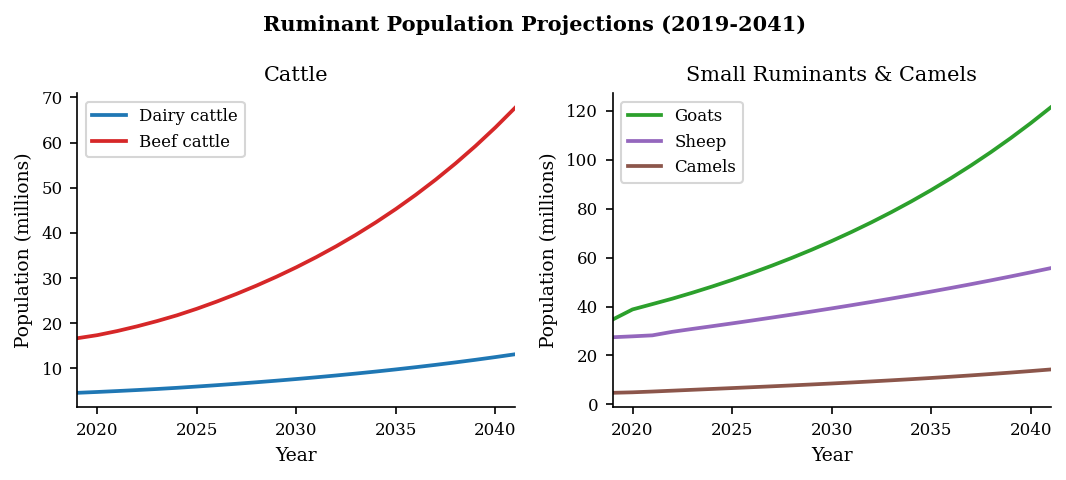
\includegraphics[width=\columnwidth]{figures/ruminant_pop.png}
  \caption{Ruminant population projections, 2019--2041. Shaded region indicates
           the 2020--2025 validation window.}
  \label{fig:rum_pop}
\end{figure}

\subsubsection{Production}

Milk production is led by dairy cattle (3.1~billion~kg in 2019 to
9.3~billion~kg by 2041; CAGR~5.12\%), followed by camels (0.99~billion~kg to
5.6~billion~kg; CAGR~8.23\%) and goats (156~million~kg to 531~million~kg;
CAGR~5.71\%). Chevon (goat meat) records the highest CAGR among all ruminant
products at 17.02\%, driven by the large baseline herd adjustment in 2020.
Beef production grows from 322~million~kg to 1.37~billion~kg (CAGR~6.82\%),
and mutton from 49~million~kg to 165~million~kg (CAGR~5.65\%). Wool production
(sheep) is modest but grows consistently (CAGR~7.25\%). Production trends are
presented in Fig.~\ref{fig:rum_prod}.

\begin{figure}[htbp]
  \centering
  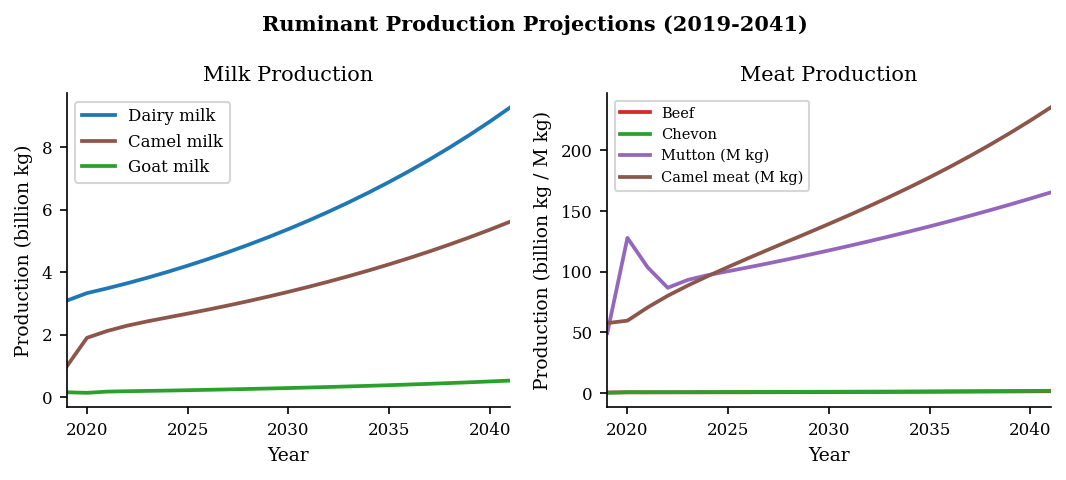
\includegraphics[width=\columnwidth]{figures/ruminant_prod.png}
  \caption{Ruminant production projections, 2019--2041.}
  \label{fig:rum_prod}
\end{figure}

\subsubsection{Feed Demand}

Beef cattle are the dominant feed consumer throughout the horizon, rising from
57.4~million~tonnes~DM to 218.3~million~tonnes~DM (CAGR~6.26\%). Dairy cattle
demand grows from 14.3~million to 41.2~million~tonnes~DM (CAGR~4.92\%).
Camel feed demand expands at CAGR~6.66\%, from 10.2~million to
42.2~million~tonnes~DM. Goat and sheep feed series begin in 2020 (no 2019
parameter baseline) and grow at CAGR 6.09\% and 3.33\% respectively over their
available range. Feed demand trajectories are shown in Fig.~\ref{fig:rum_feed}.

\begin{figure}[htbp]
  \centering
  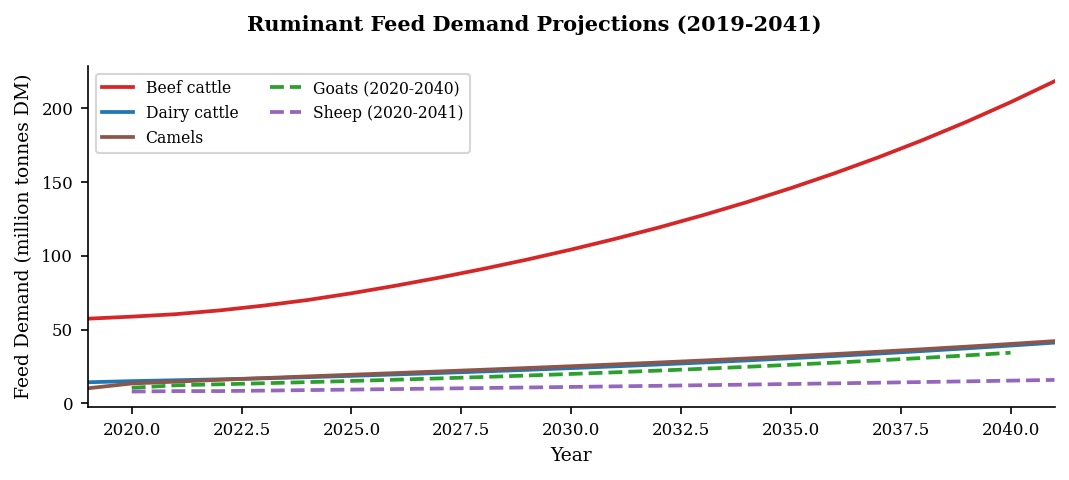
\includegraphics[width=\columnwidth]{figures/ruminant_feed.png}
  \caption{Ruminant feed demand projections, 2019--2041. Goat and sheep series
           begin in 2020; the goat 2041 value is excluded due to a data entry
           anomaly.}
  \label{fig:rum_feed}
\end{figure}

% ═════════════════════════════════════════════════════════════════════════════
\subsection{Non-Ruminant Value Chains}

\subsubsection{Population}

Indigenous poultry is the largest non-ruminant population, growing from
46.3~million to 89.3~million birds (CAGR~3.03\%). Broiler throughput and layer
flock size are relatively stable, growing at CAGR~0.43\% and 0.42\%
respectively, reflecting sector saturation assumptions. Pig and rabbit
populations expand more rapidly: pigs from 596~thousand to 2.09~million
(CAGR~5.86\%) and rabbits from 737~thousand to 3.24~million (CAGR~6.95\%).
Total apiculture hive count grows from 1.29~million to 3.49~million across all
four hive types (log, KTBH, Langstroth, box). Population trends are shown in
Fig.~\ref{fig:nonrum_pop}.

\begin{figure}[htbp]
  \centering
  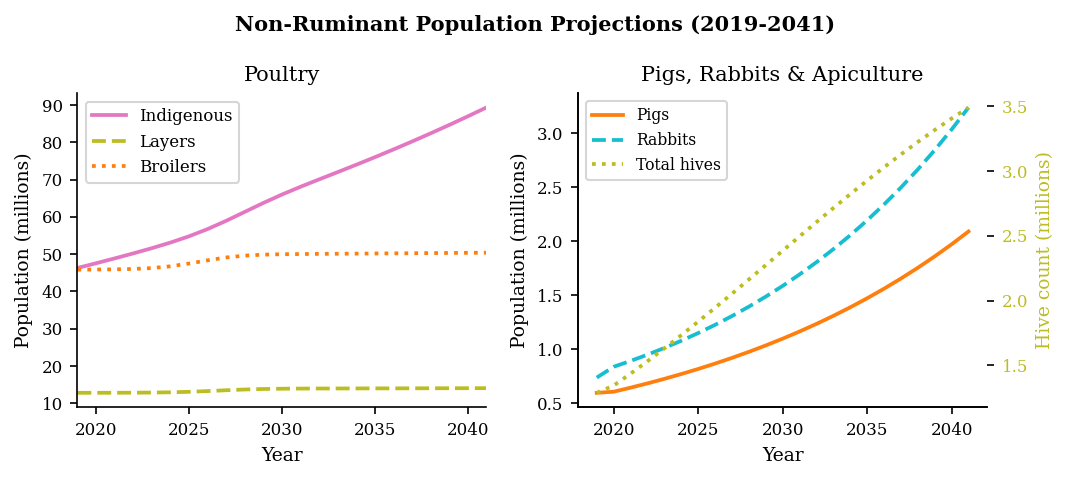
\includegraphics[width=\columnwidth]{figures/nonrum_pop.png}
  \caption{Non-ruminant population projections, 2019--2041. Right panel: pig
           and rabbit populations (left axis) and total hive count (right
           axis).}
  \label{fig:nonrum_pop}
\end{figure}

\subsubsection{Production}

Poultry meat production grows modestly from 82.4~million~kg to
109.7~million~kg (CAGR~1.31\%), consistent with the near-stable flock
projections. Egg production (layers and indigenous combined) is reported in
trays from 2020 onward — the 2019 value is excluded as it appears to reflect a
different unit convention — and grows from 180.4~million~trays to
228.7~million~trays (CAGR~1.14\%, 2020--2041). Pork and rabbit meat grow in
parallel at approximately CAGR~4.0\%. Honey production expands from
13.9~million~kg to 41.6~million~kg (CAGR~5.12\%) and beeswax from
1.4~million~kg to 6.5~million~kg (CAGR~7.35\%). Production trends are shown
in Fig.~\ref{fig:nonrum_prod}.

\begin{figure}[htbp]
  \centering
  
\includegraphics[width=\columnwidth]{figures/nonrum_prod.png}
  \caption{Non-ruminant production projections, 2019--2041. Egg production
           plotted from 2020 onward only.}
  \label{fig:nonrum_prod}
\end{figure}

\subsubsection{Feed Demand}

Poultry feed demand is the largest non-ruminant feed consumer, growing from
1.87~million~tonnes to 2.83~million~tonnes~DM (CAGR~1.89\%). Pig feed demand
grows from 448~thousand~tonnes to 1.09~million~tonnes~DM (CAGR~4.13\%). Rabbit
feed demand, though small in absolute terms (18~thousand to 53~thousand
tonnes~DM), grows at CAGR~4.94\%. Apiculture nectar demand is estimated at
852~thousand~tonnes in 2019 rising to 2.49~million~tonnes by 2041
(CAGR~5.00\%). Feed demand trajectories are shown in
Fig.~\ref{fig:nonrum_feed}.

\begin{figure}[htbp]
  \centering
  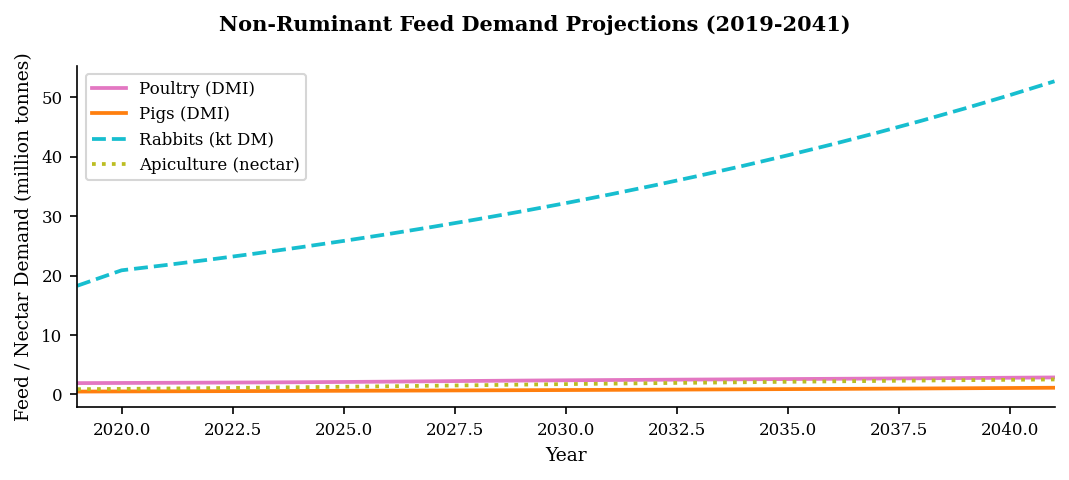
\includegraphics[width=\columnwidth]{figures/nonrum_feed.png}
  \caption{Non-ruminant feed demand projections, 2019--2041. Apiculture values
           represent nectar demand rather than DMI.}
  \label{fig:nonrum_feed}
\end{figure}

% ═════════════════════════════════════════════════════════════════════════════
\subsection{CAGR Summary}

Table~\ref{tab:cagr} summarises the CAGRs for all value chains across all three
domains. All figures are 2019--2041 unless noted.

\begin{table}[htbp]
\caption{Compound Annual Growth Rates (2019--2041)}
\label{tab:cagr}
\centering
\small
\begin{tabular}{@{}llr@{}}
\toprule
\textbf{Value Chain} & \textbf{Indicator} & \textbf{CAGR (\%)} \\
\midrule
\multicolumn{3}{@{}l}{\textit{Ruminants — Population}} \\
Dairy cattle  & Total population    & 4.93 \\
Beef cattle   & Total population    & 6.59 \\
Goats         & Total population    & 5.86 \\
Sheep         & Total population    & 3.27 \\
Camels        & Total population    & 5.15 \\
\midrule
\multicolumn{3}{@{}l}{\textit{Ruminants — Production}} \\
Dairy cattle  & Milk (kg)           & 5.12 \\
Beef cattle   & Beef (kg)           & 6.82 \\
Goats         & Milk (kg)           & 5.71 \\
Goats         & Chevon (kg)         & 17.02 \\
Sheep         & Mutton (kg)         & 5.65 \\
Sheep         & Wool (kg)           & 7.25 \\
Camels        & Milk (kg)           & 8.23 \\
Camels        & Meat (kg)           & 6.61 \\
\midrule
\multicolumn{3}{@{}l}{\textit{Ruminants — Feed Demand}} \\
Dairy cattle  & (t DM)              & 4.92 \\
Beef cattle   & (t DM)              & 6.26 \\
Goats         & (t DM, 2020--2040)  & 6.09 \\
Sheep         & (t DM, 2020--2041)  & 3.33 \\
Camels        & (t DM)              & 6.66 \\
\midrule
\multicolumn{3}{@{}l}{\textit{Non-Ruminants — Population}} \\
Poultry (indigenous) & Birds         & 3.03 \\
Poultry (layers)     & Birds         & 0.42 \\
Poultry (broilers)   & Throughput    & 0.43 \\
Pigs                 & Total         & 5.86 \\
Rabbits              & Total         & 6.95 \\
\midrule
\multicolumn{3}{@{}l}{\textit{Non-Ruminants — Production}} \\
Poultry    & Meat (kg)               & 1.31 \\
Poultry    & Eggs (trays, 2020--2041) & 1.14 \\
Pigs       & Pork (kg)               & 3.99 \\
Rabbits    & Meat (kg)               & 4.01 \\
Apiculture & Honey (kg)              & 5.12 \\
Apiculture & Wax (kg)                & 7.35 \\
\midrule
\multicolumn{3}{@{}l}{\textit{Non-Ruminants — Feed Demand}} \\
Poultry    & (t DM)                  & 1.89 \\
Pigs       & (t DM)                  & 4.13 \\
Rabbits    & (t DM)                  & 4.94 \\
Apiculture & Nectar (t)              & 5.00 \\
\bottomrule
\end{tabular}
\end{table}